% $> xelatex emv.redes-neuronales.presentacion.tex
% o bien
% $> lualatex emv.redes-neuronales.presentacion.tex
\documentclass[spanish]{beamer}

\usepackage[es-tabla]{babel}

\usepackage{graphics,tikz}
\usetikzlibrary{automata, positioning, arrows}

\usepackage{pgfplotstable}
\pgfplotsset{compat=1.16}

\usepackage{adjustbox}
\usepackage{booktabs}
\usepackage{multirow}
\usepackage{enumitem}

%%% FUENTES

\usepackage[no-math]{fontspec}
\setmainfont{Libertinus Serif}
\setsansfont{Libertinus Sans}
\setmonofont{Libertinus Mono}

\usepackage[math-style=TeX]{unicode-math}
\setmathfont{Libertinus Math}

\usepackage{pifont}
\newcommand{\cmark}{\ding{51}}%
\newcommand{\xmark}{\ding{55}}%

%%% COLORES

\definecolor{background}{HTML}{F5F5F4}
\definecolor{foreground}{HTML}{3F3F3F}
\definecolor{strings}{HTML}{ED982C}
\definecolor{operators}{HTML}{CF4818}
\definecolor{identifiers}{HTML}{9A71BA}
\definecolor{keywords}{HTML}{5486C8}
%\definecolor{keywords}{HTML}{54BFC7}
\definecolor{numbers}{HTML}{80951D}
\definecolor{comments}{HTML}{AFAFAF}

%%% LISTINGS

\usepackage{listings}

\lstset{
  numbers=left,
  belowcaptionskip=1\baselineskip,
  basicstyle=\scriptsize\ttfamily\color{foreground},
  keywordstyle=\color{keywords},
  commentstyle=\color{comments},
  stringstyle=\color{strings},
  identifierstyle=\color{identifiers},
  numberstyle=\color{foreground},
  xleftmargin=2em,
  framexleftmargin=1.5em,
  breaklines=true,
  showstringspaces=false,
  tabsize=2
}

% Bibliografía

\usepackage[sorting=none, style=apa, isbn=true]{biblatex}
\DefineBibliographyStrings{spanish}{
  urlseen = {Consultado},
  retrieved = {Consultado},
}
\addbibresource{bibliografia.bib}

%%% AJUSTES DE BEAMER

%\usefonttheme{professionalfonts}

\setlength{\leftmargini}{0cm}
\setlength{\leftmarginii}{2em}

\setbeamertemplate{navigation symbols}{}

\setbeamerfont{title}{series=\bfseries}

%\setbeamertemplate{frametitle}{\color{foreground}\vspace*{1cm}\bfseries\insertframetitle\par\vskip-6pt}
\setbeamerfont{frametitle}{series=\bfseries}
\setbeamercolor{frametitle}{fg=foreground}
\setbeamerfont{framesubtitle}{size=\normalfont\small}
\setbeamercolor{framesubtitle}{fg=foreground}

\setbeamercolor{background canvas}{bg=background}

\setbeamercolor{normal text}{fg=foreground}
\setbeamercolor{alerted text}{fg=foreground}
\setbeamercolor{block title}{fg=foreground}
\setbeamercolor{alerted text}{fg=foreground}

\setbeamercolor{itemize item}{fg=foreground}
\setbeamercolor{enumerate item}{fg=foreground}

\setbeamertemplate{itemize items}[circle]
\setitemize{
  label=\usebeamerfont*{itemize item}
  \usebeamercolor[fg]{itemize item}
  \usebeamertemplate{itemize item}
}

\setbeamercolor*{title}{fg=foreground}
\setbeamercolor{qed symbol}{fg=foreground}

\usebeamercolor[fg]{normal text}

\setbeamertemplate{footline}[frame number]
\setbeamerfont{page number in head/foot}{size=\small}

\setbeamercolor{section in toc}{fg=foreground}
\setbeamerfont{section in toc}{series=\bfseries}

\setbeamercolor{caption name}{fg=foreground}
\setbeamerfont{caption name}{series=\bfseries}

\setbeamercolor{bibliography entry note}{fg=foreground}
\setbeamercolor{bibliography entry author}{fg=foreground!40!black}

\hypersetup{
  colorlinks=true,
  citecolor=numbers,
  urlcolor=operators,
  linkcolor=foreground
}

%%% INFORMACIÓN DEL DOCUMENTO

\title{Redes neuronales artificiales}
\subtitle{Estadística Multivariante}
\author{
  Johanna Capote Robayna\texorpdfstring{\\}{}
  Antonio Coín Castro\texorpdfstring{\\}{}
  Guillermo Galindo Ortuño\texorpdfstring{\\}{}
  José María Martín Luque\texorpdfstring{\\}{}
  Luis Antonio Ortega Andrés\texorpdfstring{\\}{}
  Cristina de la Torre Villaverde
}
\institute{\normalsize Universidad de Granada}
\date{20 de enero de 2020\texorpdfstring{\\}{} \small Curso 2019-2020}

\begin{document}

\maketitle

\begin{frame}{Índice}
  \tableofcontents
\end{frame}

\section{Redes neuronales biológicas}

\begin{frame}{Redes neuronales biológicas}
  \begin{itemize}
    \item Ciencia cognitiva: estudio científico de la mente y sus procesos.
    \item Conexionismo: los fenómenos mentales pueden describirse mediante redes compuestas por unidades sencillas e interconectadas entre sí.
    \item Para entender cómo funciona una red neuronal artificial es útil comprender primero cómo funcionan las redes neuronales biológicas.
  \end{itemize}
\end{frame}

\begin{frame}{Redes neuronales biológicas}
  \begin{itemize}
    \item Neuronas: células básicas que componen el sistema nervioso.
    \item Dos partes diferenciadas: cuerpo celular y axón.
    \item Dendritas: receptores de señales.
    \item Axón: emisor de señales.
  \end{itemize}
\end{frame}

\begin{frame}{Redes neuronales biológicas}
  \begin{figure}[b]
    \centering
    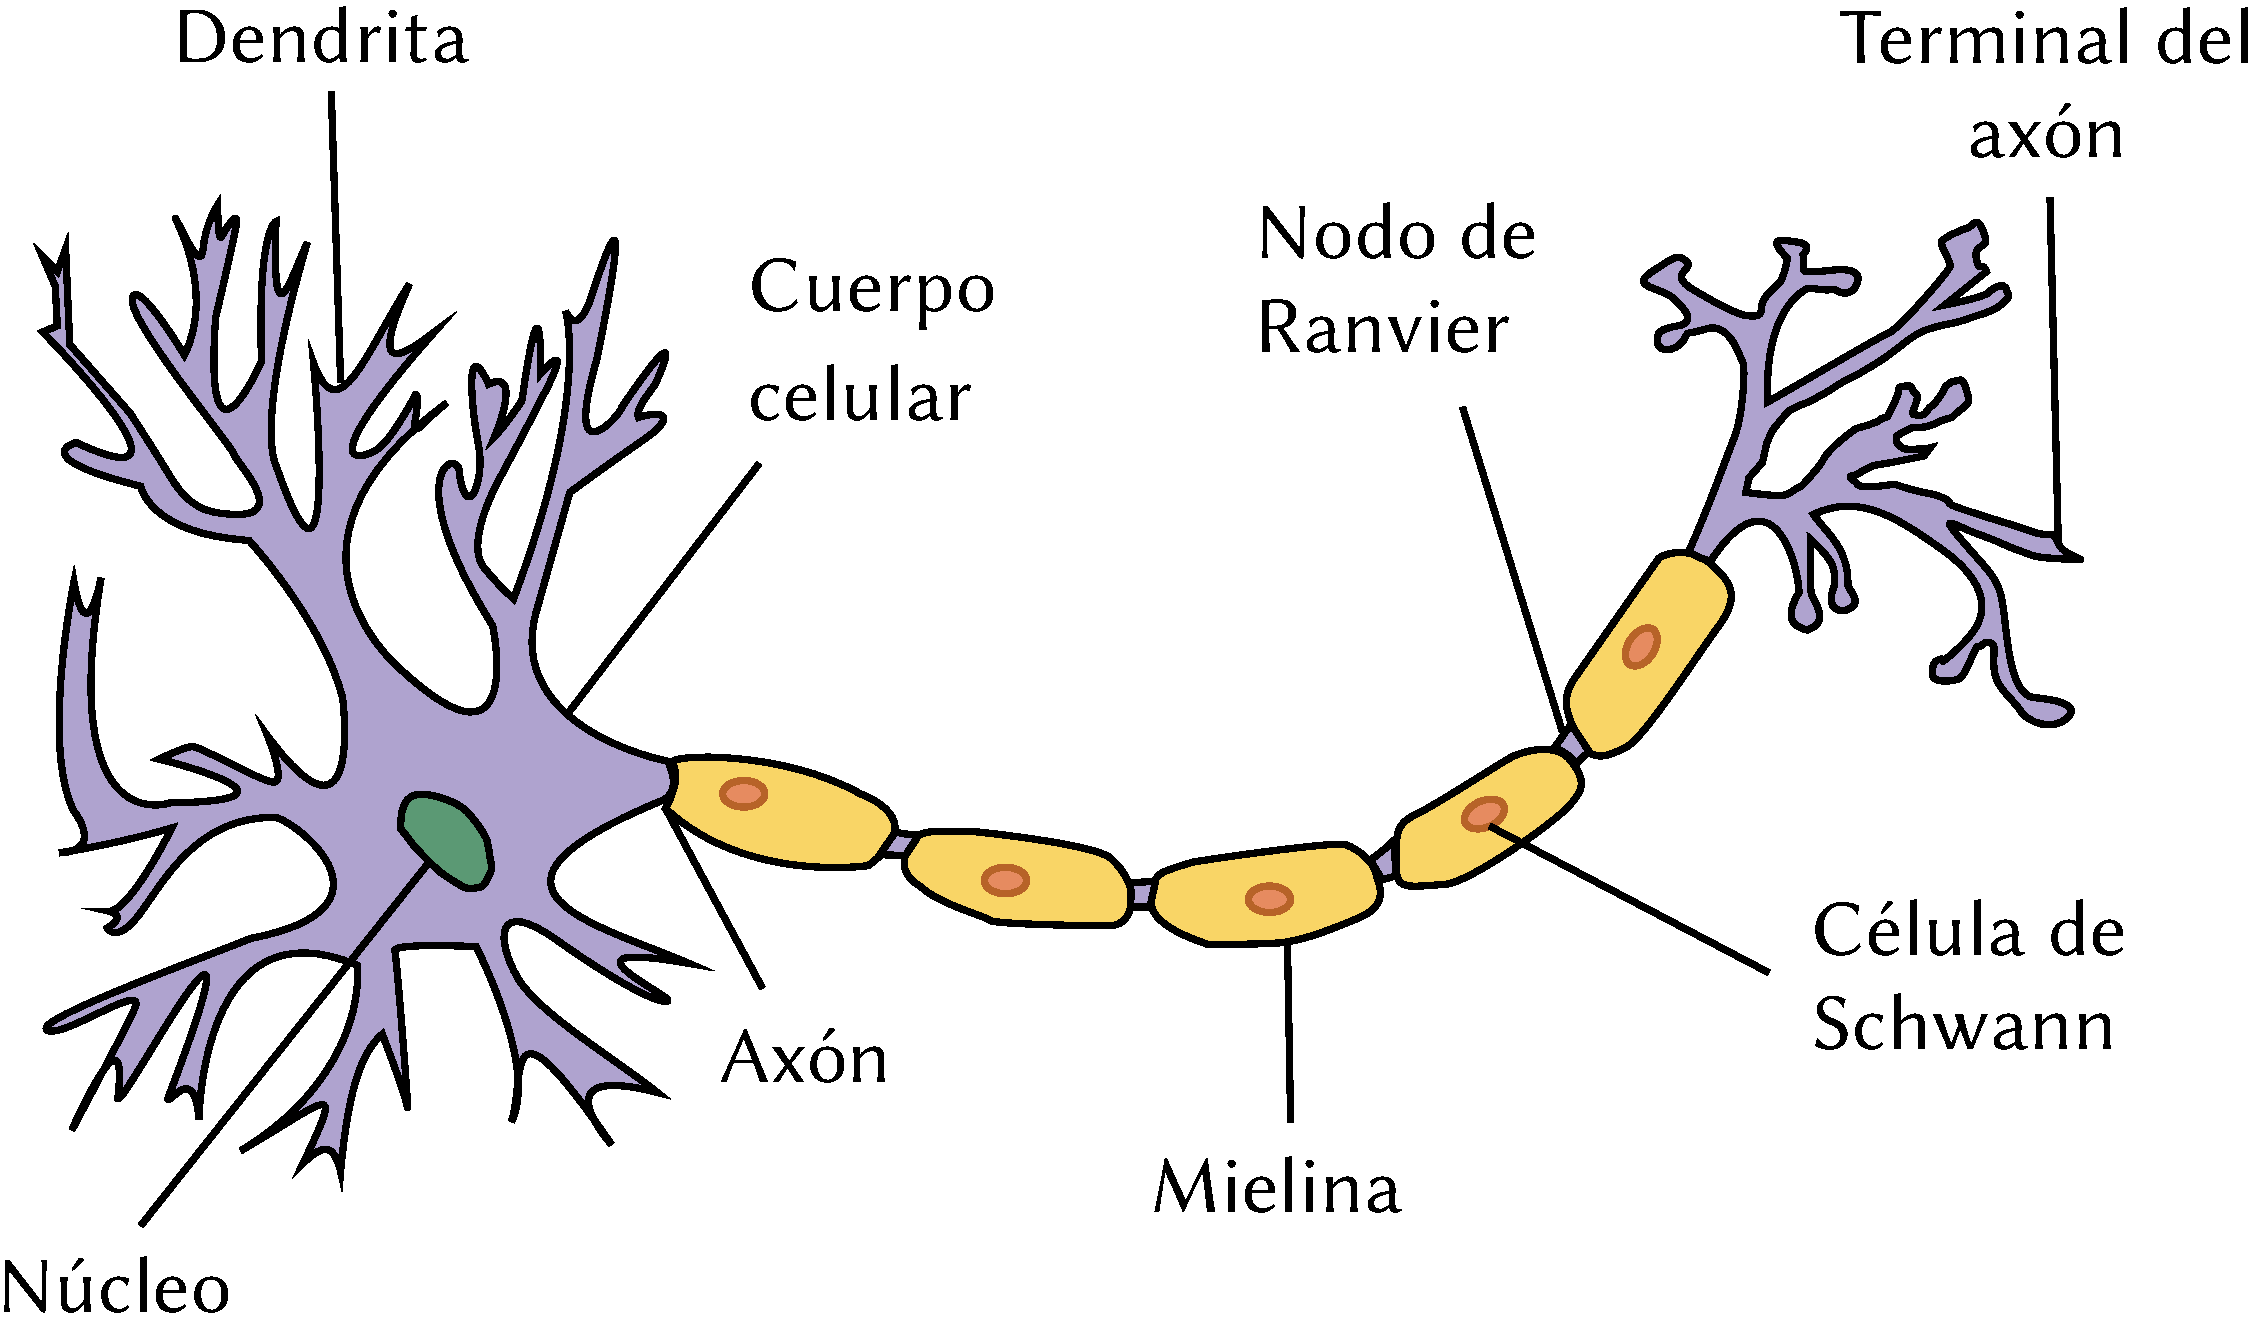
\includegraphics[width=0.7\textwidth]{img/neurona}
    \caption{Estructura de una neurona. Basada en \parencite{dhp1080_neurona_2007}.}
    \label{fig:neurona}
  \end{figure}
\end{frame}

\begin{frame}{Redes neuronales biológicas}
  \begin{itemize}
    \item Las neuronas se envían señales entre sí mediante un proceso electroquímico denominado sinapsis.
    \item La neurona presináptica (emisora) libera los neurotransmisores a través del axón y la neurona postsináptica (receptora) los capta a través de las dendritas.
    \item La tasa de envío por parte de la neurona presináptica depende de la proporción de dos tipos de sinapsis que esta reciba: \begin{itemize}
      \item sinapsis inhibidoras,
      \item sinapsis excitadoras.
    \end{itemize}
  \end{itemize}
\end{frame}

\section{Estructura y funcionamiento de las redes neuronales}

\begin{frame}{Neurona de McCulloch-Pitts}
  \begin{itemize}
    \item Modelo computacional. Múltiples entradas a una unidad de procesamiento y una sola salida.
    \item Cada entrada puede tomar el valor 0 o 1 y puede ser de tipo excitador o inhibidor. \begin{itemize}
      \item Si alguna de ellas es inhibidora y transmite el valor 1, la salida es 0.
      \item Si no hay conexiones inhibidoras activadas, se suman las entradas. Si dicha suma es mayor que el valor umbral, la salida es 1, en otro caso, 0.
    \end{itemize}
  \end{itemize}
\end{frame}

\begin{frame}{Neurona de McCulloch-Pitts}
  \begin{figure}[h]
    \centering
    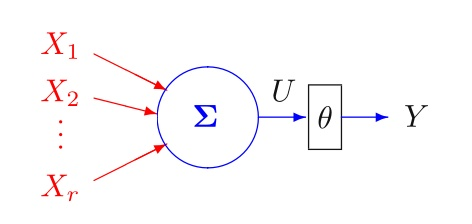
\includegraphics[width=.7\textwidth]{img/mcculloch-pitts}
    \caption{Neurona de McCulloch-Pitts con $r$ entradas binarias $X_1,\dots,X_r$, una salida binaria $Y$ y un umbral $\theta$. Extraída de \parencite{izenman_modern_2008}.}
    \label{fig:mcculloch-pitts}
  \end{figure}
\end{frame}

\begin{frame}{Neurona de McCulloch-Pitts}
  \begin{itemize}
    \item Este modelo no es adecuado para realizar un proceso de aprendizaje ya que hay que cambiar los valores de la neurona para resolver diferentes problemas.
    \item Se perdió pronto el interés en este modelo computacional y se desarrollaron otros.
  \end{itemize}
\end{frame}

\begin{frame}[t,allowframebreaks]{Referencias}
  \printbibliography[heading=none]
\end{frame}

\end{document}
